\subsection{Implementation}

For each selected track, the variables provided to the network can be found in Table~\ref{tab:rnn_vars}, and the architecture is represented schematically in Figure~\ref{fig:rnn}. The \sdip, \szip and the track category variables are the same inputs to the \textit{IP3D} algorithm. Note that the input variables, the track category, is an integer used by the \textit{IP3D} algorithm to define categories of tracks with similar reconstruction quality and resolution. The value of this variable has no physical meaning, hence this variable is embedded into a 2D continuous representation. In addition, the \textit{RNNIP} tagger is built to take in two more variables: the fraction of jet energy of each track, $\ptfrac$, and the angular separation between the track and jet axis, $\drtj$.

\begin{table}[htbp]
\small
\begin{center}
  \tabulinesep=1.5mm
  \begin{tabu}{X[-1,l,m] | X[L,m]}
\hline
   Track Variable  &  Description \\ \hline
   \hline
   \multicolumn{2}{c}{Used in \textit{IP3D} and \textit{RNNIP} tager} \\ \hline
$\sdip$	& Lifetime signed transverse impact parameter significance, $d_{0} / \sigma_{d_0}$. The detailed sign determination is documented in Sec.\ref{sec:gbb-sd0}\\ \hline 
$\szip$ & Lifetime signed longitudinal impact parameter significance, $z_{0} / \sigma_{z_0}$. The sign determination is similar to that of \sdip. \\ \hline
Category \cite{ATL-PHYS-PUB-2015-022}		& A categorization of the tracks depending on the number of observed, expected,
			 or missing hits in the different layers of the silicon pixel and strip detectors.
			 The category organizes tracks into categories of different impact parameter resolutions.\\ \hline
       \hline
       \multicolumn{2}{c}{New to the \textit{RNNIP} tagger} \\ \hline
$\ptfrac$	& The fraction of transverse momentum carried by the track relative to the jet, $p_{T}^{\rm track} / p_{T}^{\rm jet}$. \\
\hline
$\drtj$	& The angular distance between the track and the jet axis, 
						 $\sqrt{ (\phi_{\rm track} - \phi_{\rm jet})^2 +(\eta_{\rm track} - \eta_{\rm jet})^2} $.\\
\hline
\end{tabu}
\caption{Descriptions of track variables used in \textit{IP3D} and the \textit{RNNIP} tagger.}
\label{tab:rnn_vars}
\end{center}
\end{table}

The tracks within a jet has no natural ordering. Since RNN takes in sequential input, the tracks are ordered by $|\sdip|$ and passed to the LSTM cells. The output of the LSTM cells' last time-stamp is then fed into a fully-connected layer with four outputs corresponding to the $b$-jet, $c$-jet, light-jet, and $\tau$-jet probabilities ($p_b$, $p_c$, $p_{\textrm{light}}$, and $p_\tau$). The final softmax layer is connected to the dense layer in order to compute the cross-entropy loss. 

%% The RNN $b$-tagging algorithms contains a single layer of LSTM with 50 units followed by a softmax layer for classification with four outputs ($p_b$, $p_c$, $p_{\textrm{light}}$, and $p_\tau$).

%% In the context of $b$-tagging, RNNs can be used to process sets of tracks associated to a jet.  When processing a step of variables in a sequence, RNNs build probability estimates conditioned on previous step, thereby encapsulating the structure and correlations of the sequence into the RNN output. Specifically, we use Long-Short-Term-Memory (LSTM) units in recurrent layers of neurons to process features of each track in the jet and use the output of the RNN after all tracks have been processed for classification.
\begin{figure}[htbp]
  \centering
  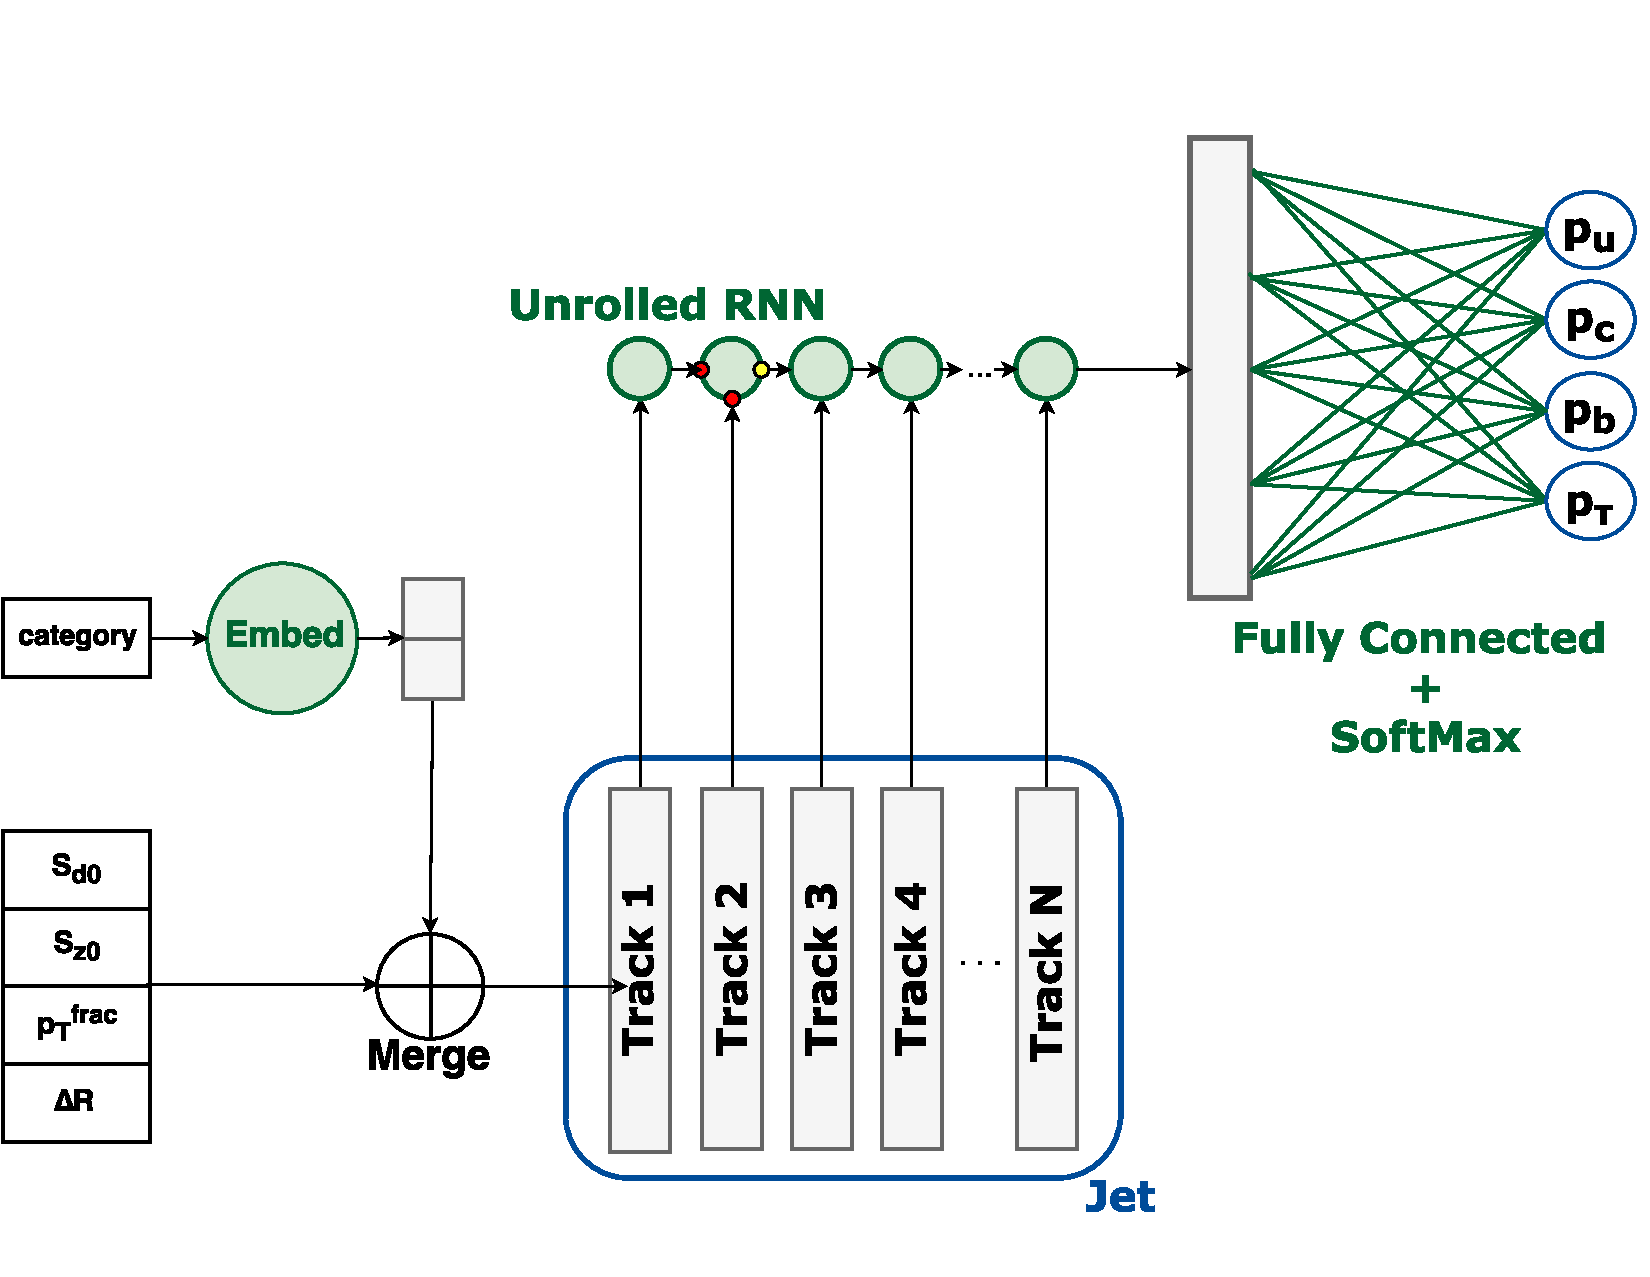
\includegraphics[width=\textwidth]{figures/RNN/RNNIP.pdf}
\caption{A schematic diagram of the RNN-based flavor-tagger.}
  \label{fig:rnn}
\end{figure}

The network was trained with 3.2 million jets and tested with an independent sample of 4 million jets. When evaluating the \textit{RNNIP}, all tracks satisfying the quality criteria listed above are used, although for the sake of training the sequence was truncated at 15 tracks. Since the fractions of the different flavor jets in $t\bar t$ sample are not even and the jet \pt distributions are different for different flavors, the jet \pt spectra and normalizaiton of $b$-jets and $c$-jets were reweighted to those of the light-jet to down-sample the light jets and train the neural network to be indifferent to the flavor specific \pt distributions. The entire network was trained for 50 epochs using \textsc{Keras}~\cite{keras} with the \textsc{Theano}~\cite{theano} backend and the Adam optimizer~\cite{ref:ADAM}. The \textit{RNNIP} tagger performance against \textit{IP3D} shown in Sec.\ref{sec:rnn-result-rnn} is trained with $t\bar{t}$ for simplicity, while the \textit{RNNIP} used for combination with other taggers as shown in Sec.\ref{sec:rnn-result-combination} is trained with a hybrid of $t\bar{t}$ and Z' sample to cover a wider range of \pt and analyses need.

Several variations of the architecutres and training procedures were considered but similar or worse tagger performance:
\begin{enumerate}
\item Ordering tracks by $|\sdip^2 + \szip^2|$ or $\pt$
\item Removing the 2D track category emdedding
\item Using Gated Recurrent Units (GRU) ~\cite{ref:GRU,cho14}, a recent variant of LSTM, as the cell units of the RNN
 
\end{enumerate}

